\documentclass[conference]{IEEEtran}
\IEEEoverridecommandlockouts
% The preceding line is only needed to identify funding in the first footnote. If that is unneeded, please comment it out.
\usepackage{cite}
\usepackage{amsmath,amssymb,amsfonts}
\usepackage{algorithmic}
\usepackage{graphicx}
\usepackage{textcomp}
\usepackage{xcolor}
\usepackage[utf8]{inputenc}
\def\BibTeX{{\rm B\kern-.05em{\sc i\kern-.025em b}\kern-.08em
    T\kern-.1667em\lower.7ex\hbox{E}\kern-.125emX}}
\begin{document}

\title{ Multimodal Neonatal Pain Classification Using EEG, ECG, and Respiration Signals with Subject-Level Validation\\}


\author{
\IEEEauthorblockN{
Arpit Pandey\IEEEauthorrefmark{1},
Alka Verma\IEEEauthorrefmark{1},
Vimal Mishra \IEEEauthorrefmark{1},
Yogendra Kumar Prajapati \IEEEauthorrefmark{2},~\IEEEmembership{Senior Member,~IEEE}}
\IEEEauthorblockA{
\IEEEauthorrefmark{1}Electronics Engineering,
Institute of Engineering and Rural Technology , Prayagraj, India
}

\IEEEauthorblockA{
\IEEEauthorrefmark{2}ECED,
Motilal Nehru National Institute of Technology  Allahabad, Prayagraj, India
}

\thanks{\IEEEauthorrefmark{1}Arpit Pandey: pandey07arpit@gmail.com.}
\thanks{\IEEEauthorrefmark{2}Yogendra Kumar Prajapati: yogendrapra@mnnit.ac.in ORCID: 0000-0002-6752-5667.}
\thanks{Dr. Alka Verma ORCID: 0000-0001-7192-1972.}
}

\maketitle

\begin{abstract}
Neonatal pain assessment is a critical clinical challenge, as preterm infants undergoing repeated procedural pain cannot verbally communicate their discomfort, and existing observational tools such as the Premature Infant Pain Profile (PIPP) are inherently subjective and unsuitable for continuous automated monitoring. This paper proposes a multimodal machine learning framework for objective neonatal pain classification using electroencephalography (EEG), electrocardiography (ECG), and respiration signals. A signal preprocessing pipeline was first validated on the PhysioNet Preterm Infant Cardiorespiratory Signals (PICS) dataset comprising 10 infants, where 26,208 ECG windows were successfully extracted and analysed. Multimodal pain classification was subsequently evaluated on the publicly available UCL neonatal pain dataset comprising 112 neonates and 308 recordings, using an XGBoost classifier with Leave-One-Subject-Out (LOSO) cross-validation. Two evaluation protocols were employed: a broad condition-based scheme and a stricter clinically-validated PIPP-confirmed subset. The proposed framework achieved mean subject-level LOSO AUCs of 0.929 on the PIPP-confirmed cohort (28 subjects) and 0.849 on the broad condition-based cohort (53 evaluable subjects), demonstrating multimodal physiological features can reliably classify neonatal pain under subject-independent evaluation.

\end{abstract}
\begin{IEEEkeywords}
Neonatal pain assessment, Multimodal physiological signals, Electroencephalography (EEG), XGBoost, Leave-One-Subject-Out Cross-Validation, PIPP score.

\end{IEEEkeywords}

\section{Introduction}

\subsection{Background and Motivation}

Neonates admitted to Neonatal Intensive Care Units (NICUs) are routinely subjected to numerous painful procedures, including heel lances, venipunctures, immunizations, and endotracheal suctioning. Repeated exposure to untreated or under-treated pain during this critical period of neurodevelopment has been linked to adverse long-term neurodevelopmental outcomes and altered pain perception. Because neonates lack the cognitive and verbal capacity to communicate their pain, clinicians must rely on alternative methods to assess pain accurately. Consequently, the development of reliable, objective pain assessment tools is of paramount importance to ensure adequate analgesia and mitigate the long-term consequences of neonatal pain.

\subsection{Current Clinical Assessment}

In clinical practice, neonatal pain is predominantly assessed using observational scoring systems such as the Premature Infant Pain Profile (PIPP)\cite{stevens1996pipp}, its revised version (PIPP-R)\cite{stevens2014pippr}, the Neonatal Infant Pain Scale (NIPS)\cite{lawrence1993nips}, and the Neonatal Facial Coding System (NFCS)\cite{grunau1987nfcs}.What these scales do is combine what a nurse can see — things like whether the baby's brow is furrowed or whether they're crying — with numbers from a monitor, like heart rate and oxygen levels, adjusted for how premature the baby is. During practice, the collected score depends on who is doing the scoring. Two nurses who are trained , observing the same infant at the same moment routinely assign different totals, because the judgments involved are really difficult to standardize. A nurse also cannot score pain continuously — it happens before and after a procedure, with nothing in between. This gap, together with the problem of subjectivity, makes an automated alternative worth pursuing.

\subsection{Machine Learning Approaches}

To address the limitations of manual scoring, researchers have increasingly turned to machine learning to decode neonatal pain from physiological signals. Early neurophysiological studies established that nociceptive stimuli elicit distinct cortical responses, such as nociceptive-specific event-related potentials (ERPs) in EEG. Building on this, feature-based machine learning methods have been applied to various physiological modalities, including EEG, ECG, and respiration.
Recently, several studies have leveraged the publicly available UCL neonatal dataset to develop automated pain classifiers. For instance, Hamwi \textit{et al.}(2025)\cite{hamwi2025eeg} demonstrated strong classification performance(AUC 0.94, Accuracy 82\%) using Logistic Regression restricted to the oldest gestational age group. Similarly, Roué\textit{et al.}(2025)\cite{roue2025objective} achieved an AUC of 0.90 using Gradient Boosting on the full dataset. While these studies have established strong baselines but still the differences in modalities , labeling strategies and validation methods make direct comparison difficult. This motivated us to work on strictly subject-independent evaluation of multimodal physiological features using LOSO.

\subsection{Contributions}
In this work, the proposed framework is developed using two complementary datasets. The PICS dataset is employed to validate the ECG preprocessing and feature extraction methodology, whereas the publicly available UCL neonatal pain dataset is used for multimodal pain classification and subject-level evaluation.
\begin{itemize}

\item Development and validation of an ECG preprocessing and heart-rate variability (HRV) feature extraction pipeline using the PICS dataset.

\item Construction of a multimodal neonatal pain classification framework integrating EEG spectral features, ERP features, ECG features, and respiration features extracted from the UCL dataset. While integrating EEG, ECG, and respiration for the first time in a fully multimodal framework evaluated with strict LOSO cross-validation.

\item Subject-independent evaluation using Leave-One-Subject-Out (LOSO) cross-validation, with model's performance evaluated on unseen newborn from the available dataset .


\end{itemize}

\section{Related Work}

\subsection{Clinical Pain Assessment in Neonates}

The assessment of pain in neonates remains a challenging clinical task because newborn infants cannot verbally communicate pain. Consequently, observational pain assessment scales have become the clinical standard for evaluating procedural pain in neonatal intensive care units (NICUs). Among these, the Premature Infant Pain Profile (PIPP)~\cite{stevens1996pipp} and its revised version (PIPP-R) are the most widely adopted. In practice, clinicians scoring pain on these scales are simultaneously watching the baby's face, reading the bedside monitor, and accounting for how premature the infant is — all folded into a single composite number that is meant to stand in for something that cannot be directly measured.

These tools have become clinical standard largely because nothing better existed, not because they are objectively reliable. When the same infant is scored by two different nurses, the results often disagree. And because scoring requires active observation, it simply cannot happen continuously — there are always gaps in the record during which a baby's pain state is unknown. Clinical assessment can also be influenced by gestational maturity, neurological development, and the administration of analgesics, motivating the search for objective physiological biomarkers capable of providing automated pain assessment.

\subsection{Physiological Biomarkers for Neonatal Pain}

Advances in physiological monitoring have enabled the investigation of objective biomarkers associated with neonatal pain. Electroencephalography (EEG) provides direct measurements of cortical activity and has been shown to exhibit characteristic nociceptive event-related potentials (ERPs) following painful stimulation. The pioneering work of Slater \textit{et al.}~\cite{slater2008cortical} demonstrated that noxious procedures evoke reproducible cortical responses even in premature infants, establishing EEG as an important modality for neonatal pain assessment.

The body reacts more profoundly to pain than the face. When a needle touches a baby's heel, the speed of heart increases, the beat-to-beat timing becomes less regular, and the pattern of breathing changes sometimes subtly, sometimes dramatically. These autonomic signals can be measured through the ECG and a respiration belt. Pain results irregulation in heart rate and heart-rate variability (HRV)\cite{taskforce1996hrv} that capture a dimension of the pain response which facial scoring completely misses.
However, each individual modality is subject to motion artifacts, developmental variability, and environmental influences.Recent studies have therefore increased exploring multimodal approaches that integrate cortical and autonomic responses to obtain a more complete picture of neonatal pain~\cite{zhou2026}.

\subsection{Machine Learning for Automated Neonatal Pain Assessment}

Machine learning has become a promising approach for translating multimodal physiological recordings into objective pain assessment tools. Early work has primarily focused on handcrafted EEG features, including event-related potentials and spectral characteristics, while later work included autonomic features from ECG and respiration.

One dataset has become the most significant testing ground for this line of research — the UCL neonatal pain dataset, collected at University College London Hospital over nine years. The reason of its significance is not just its size (112 neonates, over 300 recordings) but the fact that brain activity, heart signals, and breathing were all captured simultaneously, synchronized on the point of the heel lance was performed, together PIPP scores assigned by trained clinicians.

Among recent studies, Hamwi \textit{et al.}~\cite{hamwi2025eeg} achieved an AUC of 0.94 using Logistic Regression for older gestational-age infants. And, Roué \textit{et al.}~\cite{roue2025objective} achieved an AUC of 0.90 using a Gradient Boosting classifier trained on the complete multimodal dataset, addition to these EEG-based machine learning has also been implemented for neonatal heel-lance pain~\cite{shafiee2024}, while recent reviews highlight the growing use of multimodal intelligent assessment methods~\cite{zhou2026}. These recent studies gives a valuable benchmarks but direct  numerical comparisons remain complicated because differences in datasets, labels, features, and validation procedures.

\subsection{Research Gap and Motivation}

Although recent studies have demonstrated promising performance on neonatal pain classification, several important challenges remain. Existing approaches frequently focus on a limited subset of physiological features or employ evaluation strategies that may not adequately assess subject-level generalization. In addition, relatively few studies explicitly validate their signal preprocessing pipelines prior to large-scale model development.

The approach taken here tries to address both gaps at once. Before any pain classifier was trained, the signal processing pipeline was tested independently on a separate dataset — the PhysioNet PICS database — specifically to confirm that the ECG cleaning and HRV extraction were producing sensible outputs on real neonatal recordings. Only after that validation was complete was the pipeline applied to the UCL pain data. ECG, and respiration is developed and evaluated on the UCL dataset using Leave-One-Subject-Out (LOSO) cross-validation. This way of subject-independent evaluation protocol evaluates performance on previously unseen infants in the available dataset, this provides a strict assessment than sample-level random splitting. However , evalutaion on an independent external dataset is still required to confirm broader clinical generalizability. 

\section{MATERIALS AND METHODS}

\subsection{Datasets}

\subsubsection{PICS Dataset (Pipeline Validation)}

The Pain in Infants Clinical Study (PICS)\cite{moody2001physionet} dataset was used exclusively for validation of the proposed ECG preprocessing and feature extraction pipeline. The dataset consists of continuous ECG recordings collected from 10 infants during clinically required procedures. ECG signals were sampled at 500 Hz and processed using the NeuroKit2\cite{makowski2021neurokit2} toolbox to perform signal cleaning, R-peak detection, and heart-rate variability (HRV)-analysis\cite{taskforce1996hrv}.

Unlike the UCL dataset, the PICS dataset was not used for classifier training. Instead, it served as an independent validation dataset to verify the robustness of the ECG preprocessing methodology prior to multimodal pain classification. Following preprocessing, a total of 26,208 ECG windows were successfully extracted and analyzed.
\begin{table}[ht]
\caption{PICS Dataset Overview}
\centering
\begin{tabular}{|l|c|}
\hline
Dataset & PICS \\
\hline
Subjects & 10 infants \\
Signal & ECG \\
Sampling Rate & 500 Hz \\
Windows Extracted & 26,208 \\
Purpose & ECG pipeline validation \\
\hline
\end{tabular}
\label{tab:pics}
\end{table}

\subsubsection{UCL Dataset (Pain Classification)}

The primary experiments in this study were conducted using the publicly available University College London (UCL) neonatal pain dataset\cite{jones2018ucl} obtained through the UK Data Service. The dataset contains synchronized multimodal physiological recordings acquired during clinically relevant experimental procedures.

A total of 112 neonates were included in the study, resulting in 308 successfully processed recordings out of 310 available recordings. Each recording contains synchronized EEG, ECG, and respiration signals collected during heel lance (pain), sham control, and auditory control procedures.

Pain labels were generated using both experimental condition information and Premature Infant Pain Profile (PIPP) scores. In addition to the complete dataset, a PIPP-confirmed subset was constructed by selecting recordings with clinically significant pain scores (PIPP $\geq$ 7), enabling a stricter evaluation protocol.

\begin{table}[ht]
\caption{UCL Dataset Overview}
\centering
\begin{tabular}{|l|c|}
\hline
Dataset & UCL \\
\hline
Subjects & 112 neonates \\
Processed Recordings & 308 / 310 \\
Signals & EEG, ECG, Respiration \\
Sampling Rate & 2000 Hz (EEG) \\
Pain Stimulus & Heel Lance \\
Control Conditions & Sham, Auditory \\
Labels & Condition + PIPP Score \\
Purpose & Pain Classification \\
\hline
\end{tabular}
\label{tab:ucl}
\end{table}

\subsection{Overall Framework}
The overall methodology adopted in this work is illustrated in Figure~\ref{fig:pipeline}.The framework consists of five sequential stages: data acquisition, physiological signal preprocessing, multimodal feature extraction, feature matrix construction, and subject-independent pain classification using XGBoost\cite{chen2016xgboost} with Leave-One-Subject-Out (LOSO)-cross-validation\cite{varoquaux2018crossvalidation}.

\begin{figure}[!t]
\centering
\includegraphics[width=\columnwidth]{pipeline.png}
\caption{Overview of the proposed framework.}
\label{fig:pipeline}
\end{figure}

\subsection{Signal Processing}
EEG preprocessing involved spectral analysis using Welch's power spectral density estimation\cite{welch1967psd}, extraction of delta, theta, alpha and beta band power, computation of event-related potential (ERP) characteristics, and estimation of Global Field Power (GFP)\cite{lehmann1980gfp}.The raw multimodal signals are illustrated in Figure~\ref{fig:uclsignals}

\begin{figure}[t]
\centering
\includegraphics[width=\columnwidth]{ucl_single_file_signals_paper.png}
\caption{Representative multimodal physiological recording from the UCL dataset showing synchronized EEG, ECG, and respiration signals aligned to stimulus onset.}
\label{fig:uclsignals}
\end{figure}


\subsection{Feature Extraction}

Following modality-specific preprocessing, quantitative physiological features were extracted from the EEG, ECG, and respiration signals to construct a unified multimodal feature representation for pain classification.
Following feature extraction, a total of 69 features were retained after preprocessing, yielding a unified feature vector per recording.

For the ECG modality, heart rate (HR) and Heart Rate Variability (HRV) features were computed from the detected R-peaks, including MeanNN, SDNN, RMSSD, pNN50, LF power, HF power, and the LF/HF ratio. EEG features comprised spectral band power (Delta, Theta, Alpha, and Beta) together with event-related potential (ERP) descriptors extracted from the post-stimulus response window. Respiration features were represented using statistical descriptors, including the mean and standard deviation within the analysis window.

Figure~\ref{fig:eda} presents an exploratory analysis of the ECG-derived physiological features extracted from the PICS dataset. The distributions of HR, RMSSD, and SDNN across individual infants demonstrate both inter-subject variability and consistent physiological trends, while the feature correlation matrix highlights the relationships among the extracted HRV metrics. This analysis provides additional validation of the extracted feature set prior to multimodal classification.

Table~\ref{tab:features} summarizes the complete set of features extracted from each physiological modality and used to construct the final multimodal feature matrix.

\begin{table*}[ht]
\caption{Extracted Features}
\centering
\begin{tabular}{|l|l|}
\hline
Modality & Features \\
\hline
EEG &
Delta, Theta, Alpha, Beta Band Power,
ERP Peak,
ERP Mean,
Global Field Power \\
\hline
ECG &
Pre/Post Heart Rate,
Heart Rate Change,
MeanNN,
SDNN,
RMSSD,
LF,
HF,
LF/HF Ratio \\
\hline
Respiration &
Mean,
Standard Deviation \\
\hline
\end{tabular}
\label{tab:features}
\end{table*}

\begin{figure}[t]
\centering
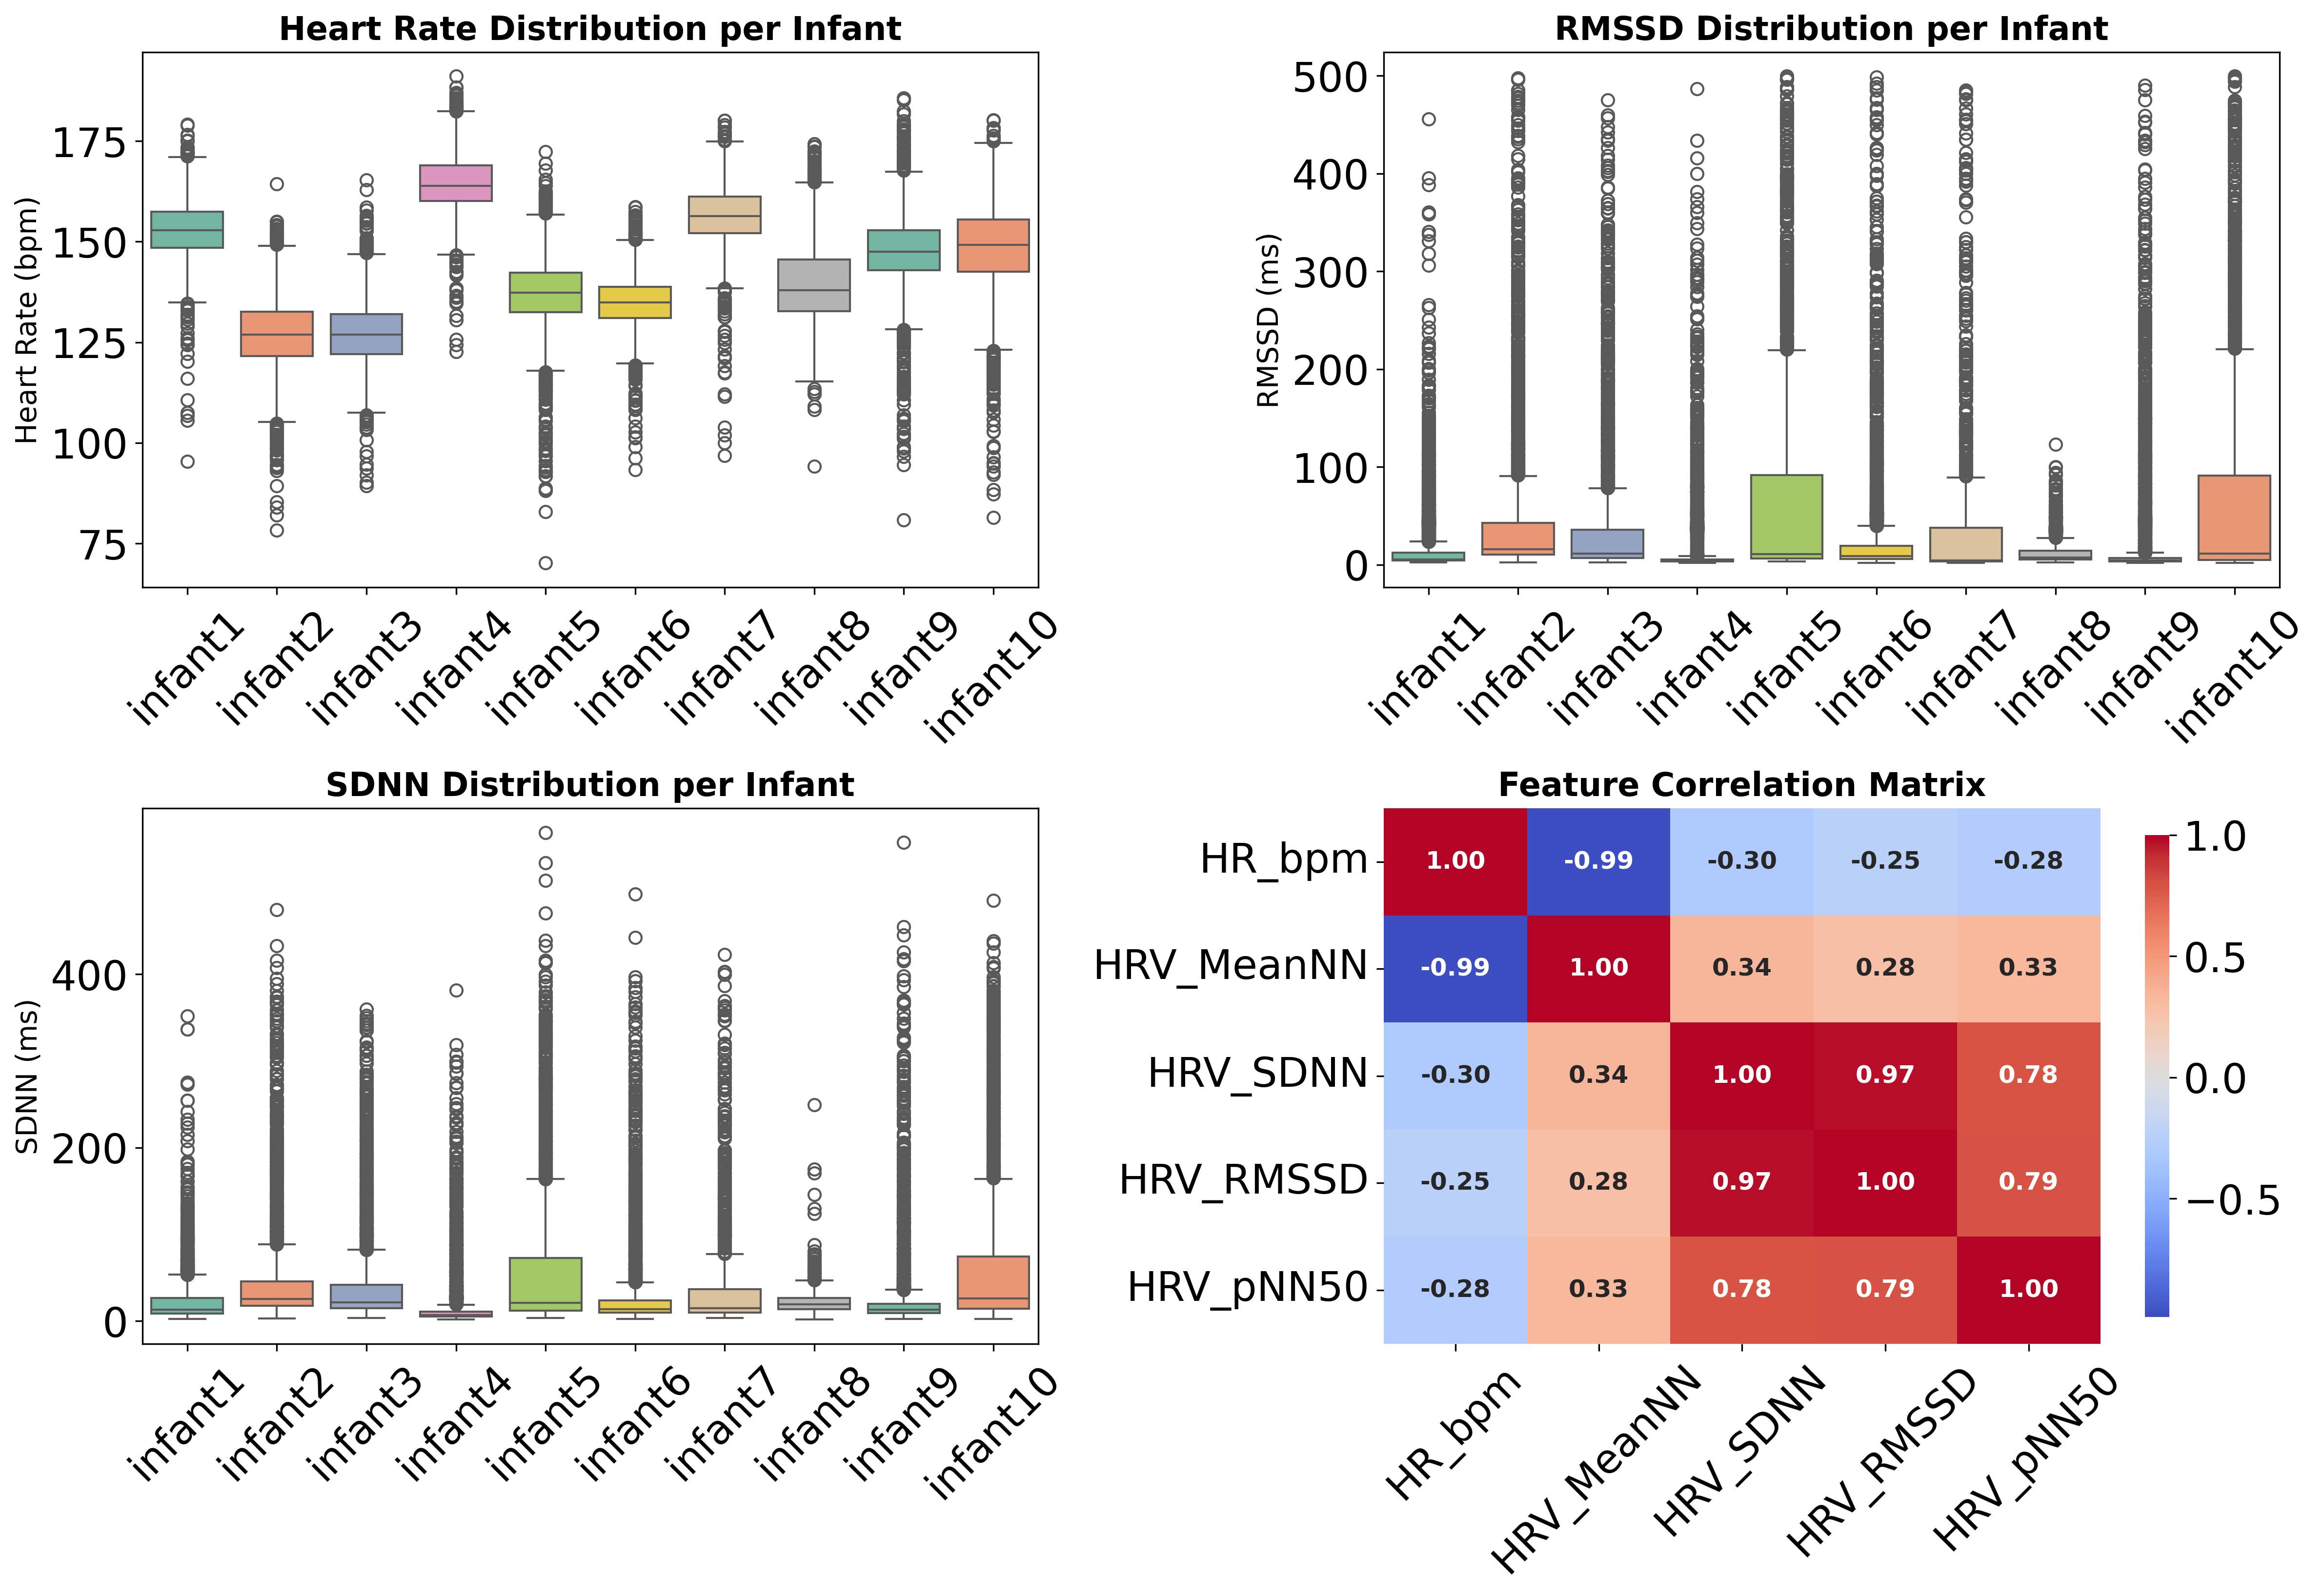
\includegraphics[width=\columnwidth]{cross_infant_eda_new.png}
\caption{Exploratory analysis of ECG-derived HRV features extracted from the PICS dataset. Box plots show inter-subject variability in heart rate, RMSSD, and SDNN across 10 infants, alongside the feature correlation matrix.}
\label{fig:eda}
\end{figure}

\subsection{Classification}
Feature standardization was performed independently within each LOSO fold using StandardScaler to prevent information leakage. Using XGBoost classifier we kept the estimators at 200 , maximum tree depth of 4, and a learning rate of 0.05, with class weighting calculated from the training potion of each fold to account for class imbalance. The random state was fixed at 42 and the final feature representation includes total 69 features. 
For each held-out subject, subject level ROC-AUC calculated using predicated probabilities , while F1 score is calculated from corresponding discrete class predictions. The primary AUC has been reported in this study represents the arithmetic mean of the subject level LOSO AUCs, by giving equal weight to each evaluated subject. 95\% Confidence Intervals calculated across the subject level AUC values. Pooled out-of-fold predictions were additionally used to construct the aggregate ROC curves in Fig.~\ref{fig:roc}; therefore the pooled AUC values differ from the mean subject-level AUCs reported in Table~\ref{tab:results}.
The computational requirements recorded during the LOSO analysis. The reported Across evaluated folds, mean training time was 0.235s per held-out subject, with a median of 0.213s , while reported mean inference time was 0.00225s, with a median of 0.00204s.
All the experiment conducted on a windows system with a 12 core Intel processor using Python 3.10.20, scikit-learn 1.7.2 and XGBoost 3.2.0.

\section{Experimental Results}

Before integrating into multimodal pain classification, the proposed ECG preprocessing and feature extraction pipeline was independently validated using the PICS dataset. The aim of this experiment was to validate the ECG processing methodology before applying it to larger multimodal UCL dataset.

Every recording was filtered, heartbeats located, and HRV features extracted from 60-second windows. Across all ten infants we got 26,208 valid windows , enough to confirm the pipeline behaved consistently across subjects with different recording lengths and heart rates.

Figure~\ref{fig:pics_validation} shows a representative preprocessing example. The upper panel presents the cleaned ECG signal together with automatically detected R-peaks, while the lower panel shows the corresponding heart-rate profile derived from the detected cardiac cycles. The successful identification of R-peaks in neonatal ECG recordings, despite the presence of motion artefacts and physiological noise, demonstrates the robustness of the proposed preprocessing pipeline. The extracted HRV features subsequently formed the ECG component of the multimodal feature matrix used for pain classification.
\begin{figure}[!t]
\centering
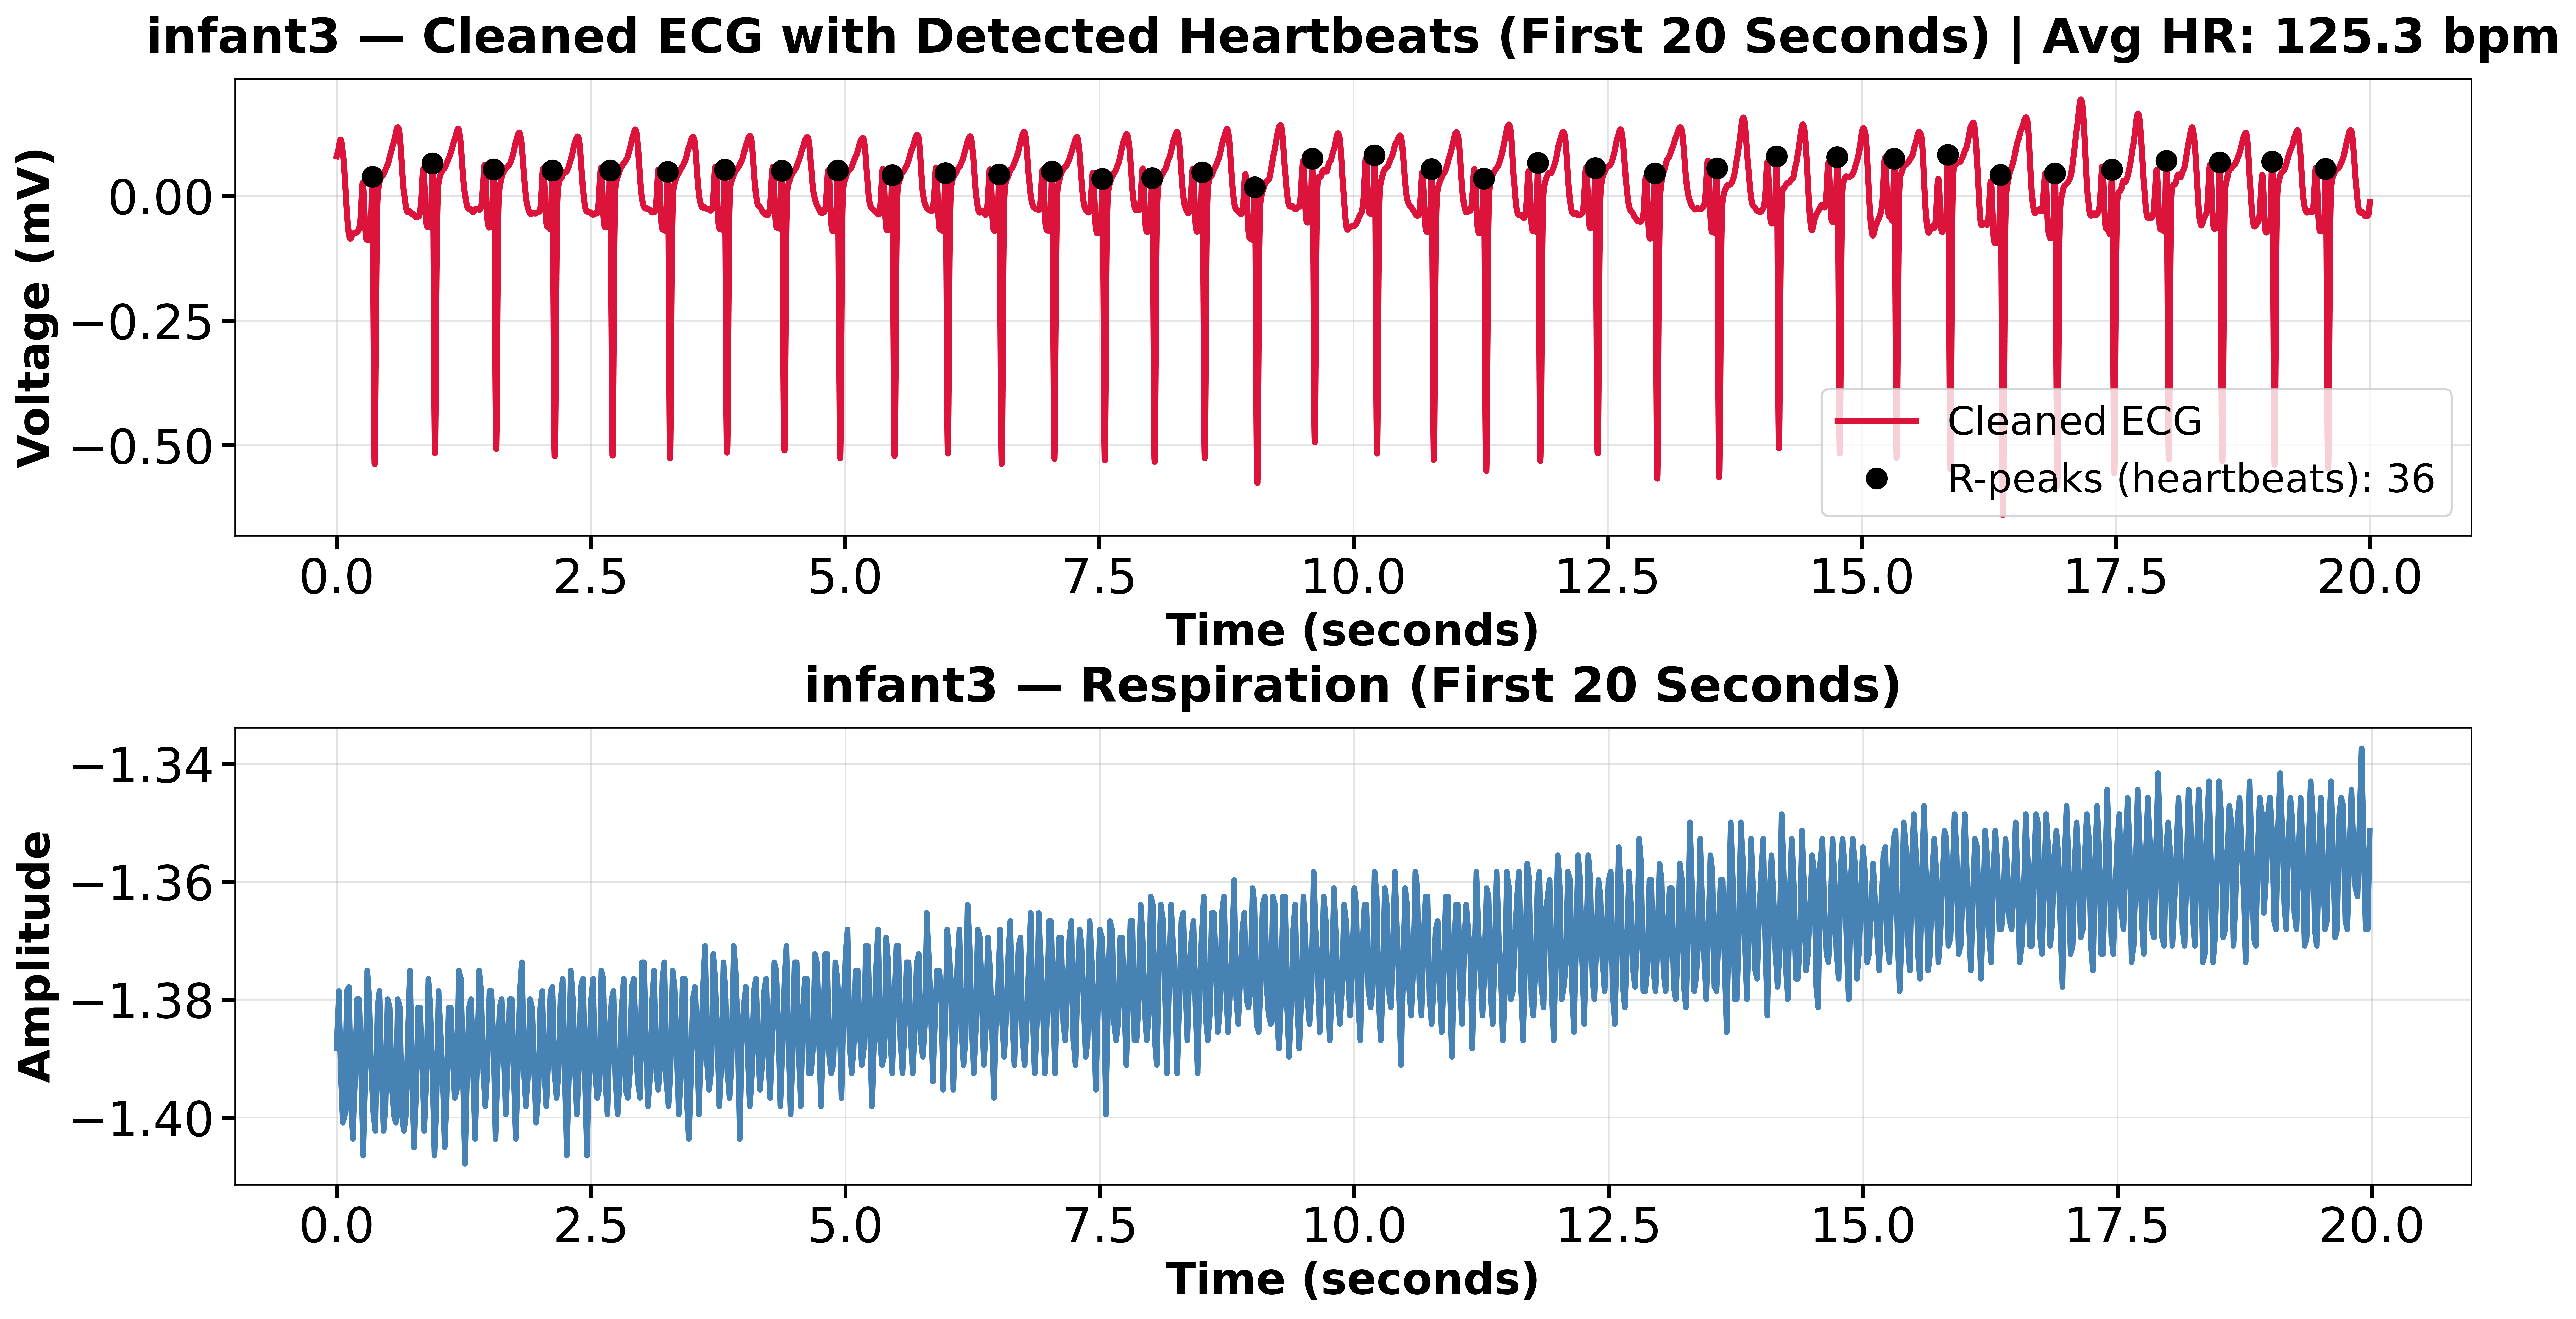
\includegraphics[width=\columnwidth]{infant3_ecg_resp_peaks_paper.png}
\caption{ Validation of the ECG preprocessing pipeline using the PICS dataset. The cleaned ECG waveform with automatically detected R-peaks demonstrates reliable heartbeat detection following signal preprocessing, enabling robust heart rate and heart rate variability (HRV) feature extraction.}
\label{fig:pics_validation}
\end{figure}

\subsection{Validation of the ECG Preprocessing Pipeline Using the PICS Dataset}

Before any pain-labelled data was used, the pipeline ran against the PICS recordings as a test. Ten infants across hundreds of hours of continuous monitoring gave a realistic check that the cleaning and peak detection produced sensible results, R-peak detection, and HRV analysis, yielding 26,208 ECG windows. Figure~\ref{fig:pics_validation} illustrates a representative result: automatically detected R-peaks on cleaned ECG demonstrate reliable heartbeat identification despite motion artefacts, confirming pipeline robustness for neonatal signals.

\subsection{Multimodal Pain Classification on the UCL Dataset}

The proposed multimodal framework was evaluated on the UCL neonatal pain dataset using Leave-One-Subject-Out (LOSO) cross-validation to ensure subject-independent assessment. EEG, ECG, and respiration features extracted from each recording were combined into a unified feature vector and classified using an XGBoost classifier.

Two evaluation protocols were considered. The first used broad condition-based labels (heel lance versus control), resulting in 53 evaluable subjects. The second used a clinically validated subset containing recordings with available Premature Infant Pain Profile (PIPP) scores, where samples with PIPP $\geq$ 7 were considered pain events, resulting in 28 subjects.Quantitative performance under both evaluation protocols is summarized in Table IV.

The quantitative performance under both evaluation protocols is summarized in Table~\ref{tab:results}.

\begin{table}[t]
\caption{Classification Performance Using LOSO Cross-Validation}
\centering
\begin{tabular}{lccc}
\hline
Evaluation Group & Subjects & Mean AUC [95\% CI] & Mean F1-score \\
\hline
Broad Condition-based & 53 & $0.849 \pm 0.287$ [0.770, 0.928] & $0.475 \pm 0.450$ \\
PIPP-confirmed & 28 & $0.929 \pm 0.178$ [0.859, 0.998] & $0.452 \pm 0.438$ \\
\hline
\end{tabular}
\label{tab:results}
\end{table}
The mean subject-level AUCs in Table IV were 0.849 and 0.929, with 95\% CIs of [0.770, 0.928] and [0.859, 0.998], respectively. AUC is based on the continuous prediction scores across thresholds whereas F1-score depends on a fixed classification threshold. The small and varying class composition of held-out LOSO test sets therefore makes F1 sensitive to individual prediction errors. Fixed-threshold sensitivity analysis gave maximum observed F1-scores of 0.672 at 0.40 for the broad protocol and 0.703 at 0.20 for the PIPP-confirmed protocol; these were not used as optimized test-set thresholds.

Figure~\ref{fig:roc} shows pooled out-of-fold ROC curves, showing AUCs of 0.806 and 0.810, respectively, that differ from the mean subject-level AUCs in Table IV because pooled predictions weight subjects by their available samples. The PIPP-confirmed result is based on only 28 subjects; therefore, the findings remain limited to the available cohort and require independent validation on larger, multi-centre datasets.

\begin{figure}[!t] 
\centering
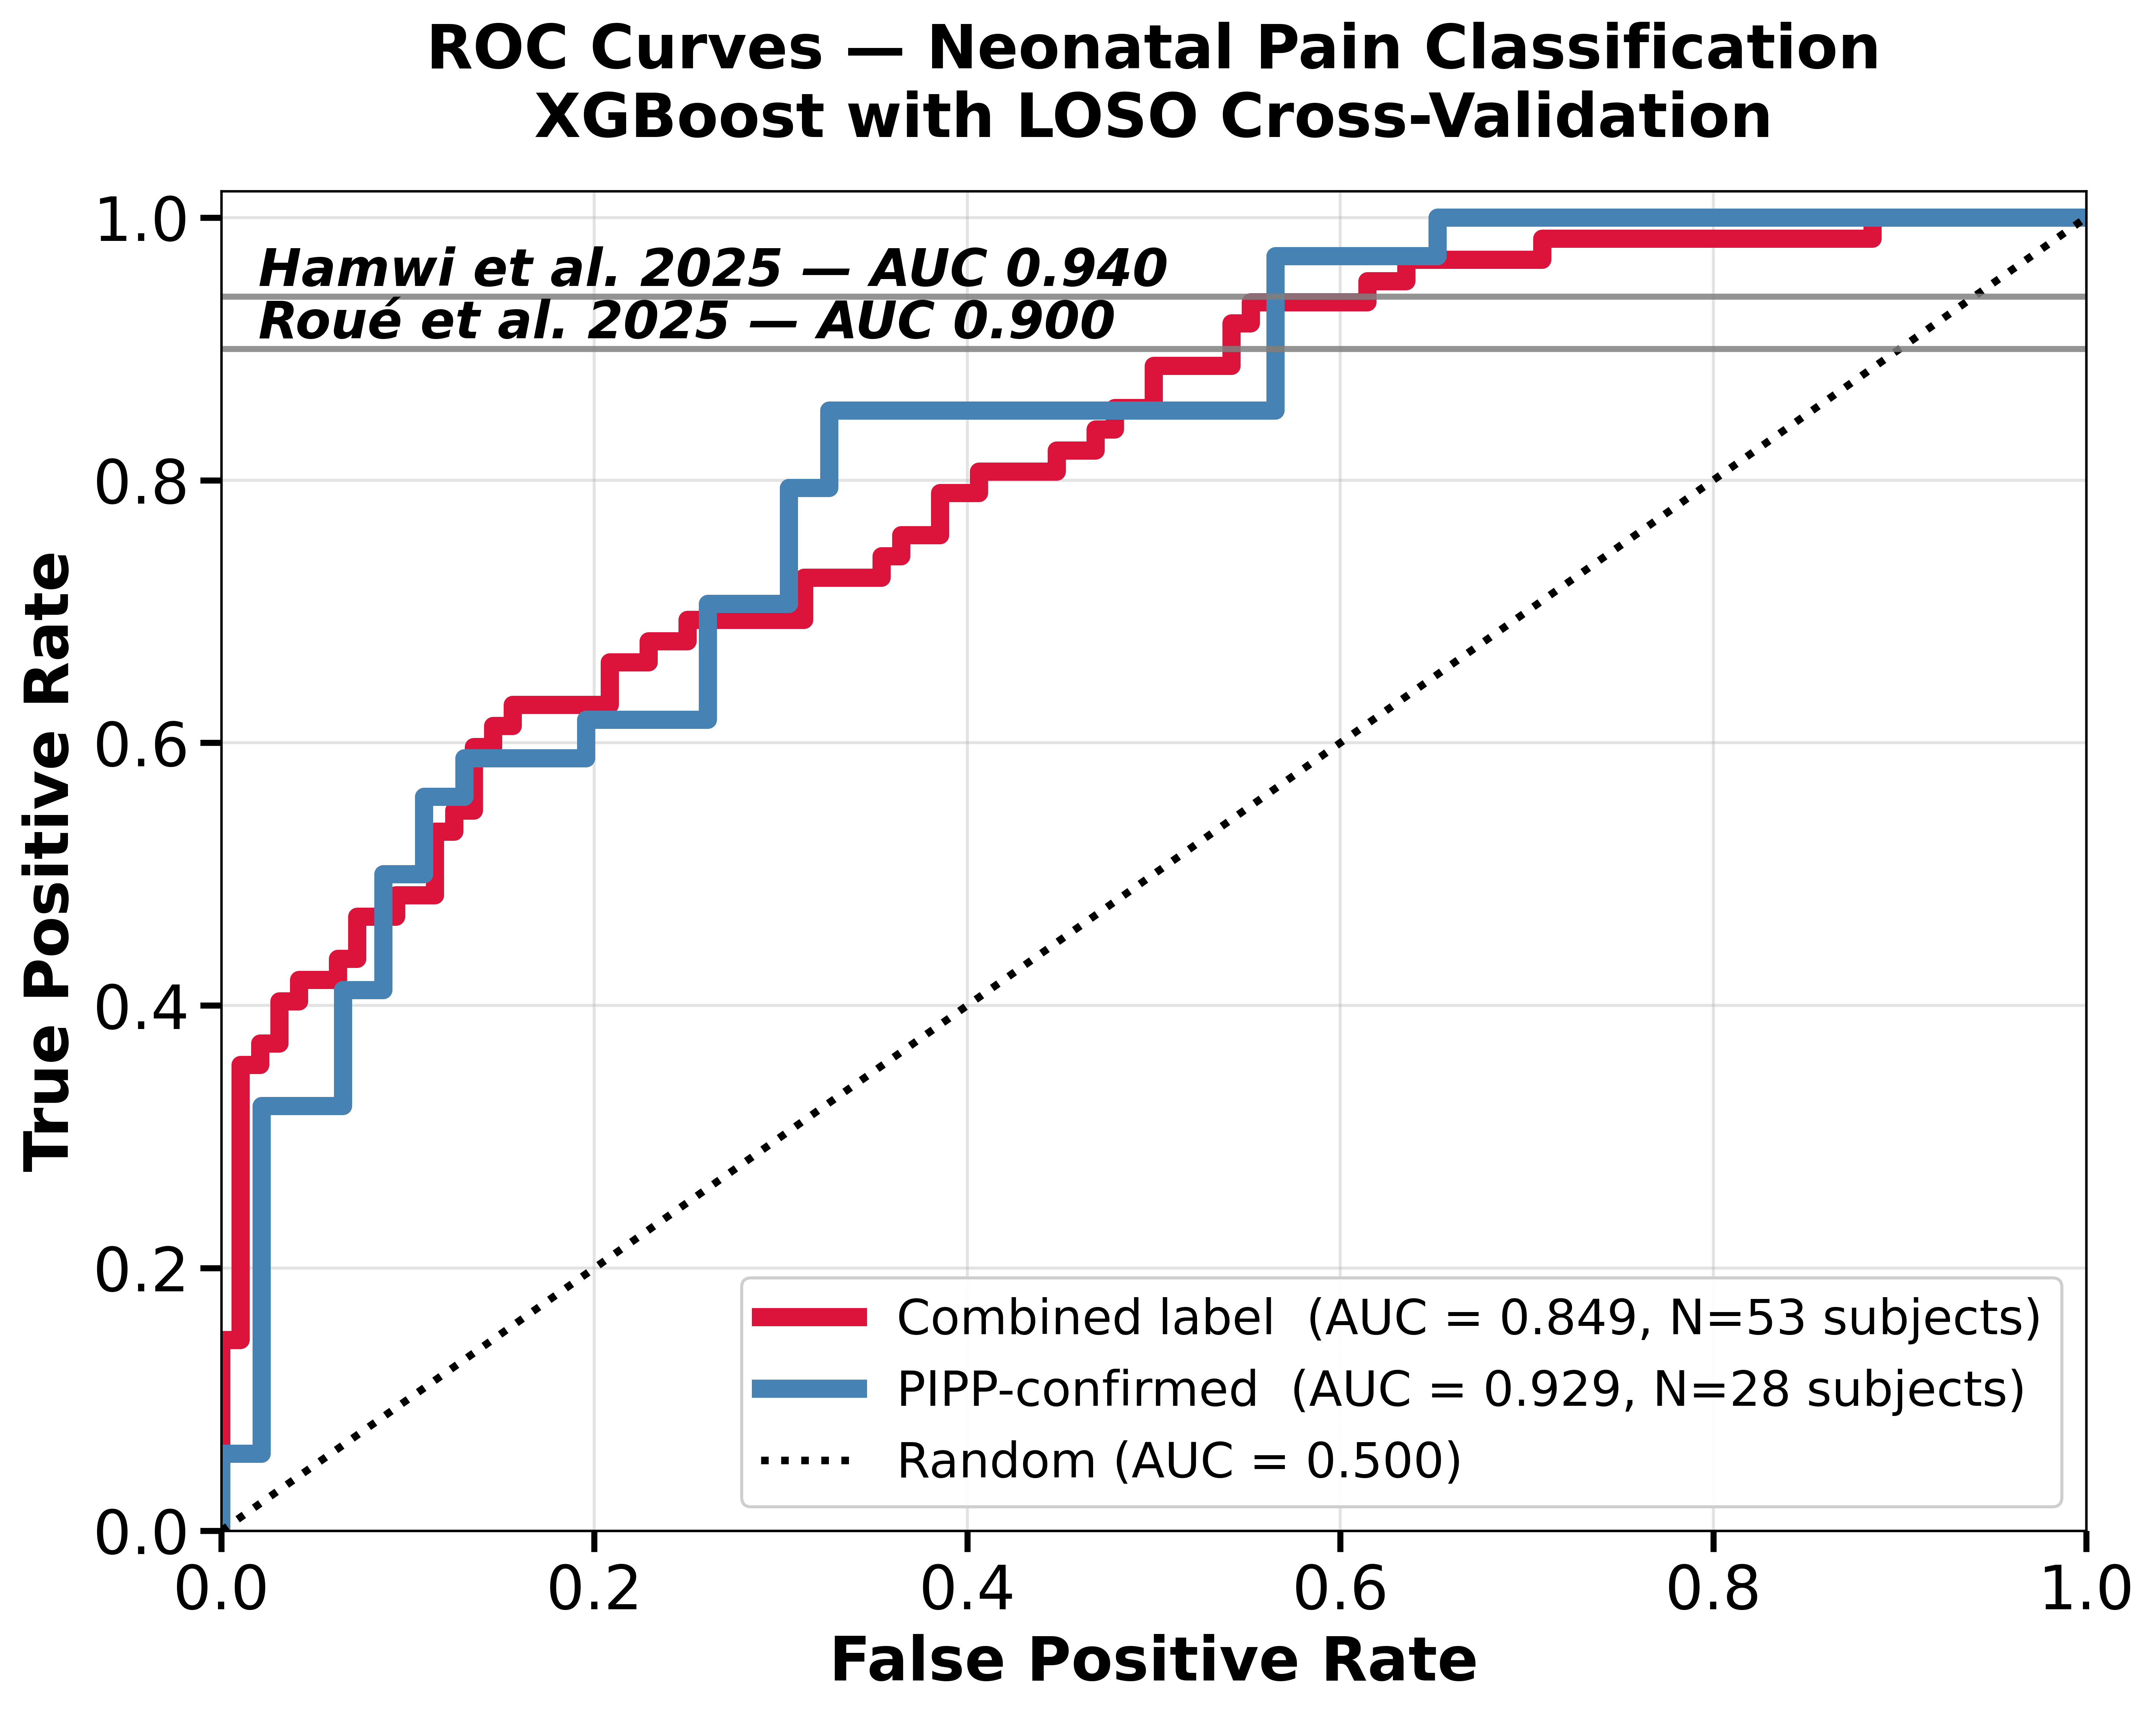
\includegraphics[width=\columnwidth]{roc_dual_final_paper.png}
\caption{ROC curves using pooled out of fold predictions applying LOSO evaluation. Pooled AUCs were 0.806 and 0.810 for the broad condition-based and PIPP-confirmed protocols, respectively.}
\label{fig:roc}
\end{figure}


\subsection{Comparison with Existing Methods}

The proposed framework was compared with recent studies that employed the same UCL neonatal pain dataset. Table~\ref{tab:comparison} summarizes the reported performance of representative machine learning approaches.

\begin{table}[t]
\caption{Comparison with Recent Studies}
\centering
\begin{tabular}{lccc}
\hline
Study & Classifier & Validation & AUC \\
\hline
Hamwi et al.\cite{hamwi2025eeg} & Logistic Regression & LOSO & 0.94$^{\dagger}$ \\
Roué et al.\cite{roue2025objective} & Gradient Boosting & Subject-level & 0.90 \\
Proposed Method & XGBoost & LOSO, PIPP-confirmed & \textbf{0.929}$^{*}$ \\
\hline
\multicolumn{4}{l}{$^{\dagger}$Restricted to infants with gestational age $\geq 34$ weeks.}\\
\multicolumn{4}{l}{$^{*}$Mean subject-level AUC across 28 PIPP-confirmed evaluable subjects.}\\
\end{tabular}
\label{tab:comparison}
\end{table}

There is a limitation in the Direct numerical comparison because of differences in Datsets, label definitions, feature sets, and AUC aggregation. Achieved value of 0.929 represents the mean subject-level AUC across 28 PIPP-confirmed evaluable subjects.

\section{Discussion}

Our multimodal framework shows that EEG, ECG, and respiration features have useful information for neonatal pain classification using subject-level LOSO evaluation. The experiment with the PICS dataset provided an independent check for the ECG preprocessing and HRV extraction pipeline before its use in the multimodal analysis.

Difference between AUC and F1 highlights the effect of the evaluation setting. AUC is evaluating continuous prediction scores across thresholds, whereas F1 is relying on a fixed classification threshold.Even with the small and varying held-out samples, whixh causes errors on individual prediction that can produce strong changes in F1 even when AUC is relatively high.And the threshold sensitivity analysis verifies this interpretation.

The higher mean AUC of 0.929 achieved by PIPP-confirmed protocol compared with 0.849 for the broad condition-based protocol, while the proposed two protocols differ in label definitions and evaluable populations. This result supports the potential of clinically informed labels for multimodal neonatal pain classification, although the PIPP-confirmed analysis was limited to 28 subjects. LOSO provides subject-independent evaluation within the available cohort, while the important next step would be validation on larger independent and multi-centre neonatal datasets .Whereas the most important future work would be Detailed model interpretability using explainable machine learning methods such as SHAP .

\textit{Limitations:} The scale of this analysis is limited by PIPP score availability (79 of 112 subjects have scores) and the requirement for mixed-class test sets in LOSO. In particular, the PIPP-confirmed analysis is available for only 28 subjects, that limits generalisability to the available cohort. External validation on independent and larger multi-centre neonatal cohorts, together with model interpretability using explainable machine learning techniques, remains future work.

\section{Conclusion}

We presented a multimodal machine learning framework for automated neonatal pain classification using EEG, ECG, and respiration signals.The PICS dataset has been used to first validated ECG preprocessing and HRV extraction workflow , followed by multimodal pain classification on the UCL neonatal pain dataset using XGBoost with LOSO cross-validation.

The broad condition-based protocol achieved a mean subject-level AUC of 0.849 across 53 evaluable subjects, while the PIPP-confirmed protocol achieved 0.929 across 28 subjects. These metrics prove that the multimodal feature set hold strong information under subject-independent evaluation, while differences between the protocols should be interpreted in the context of their different label definitions and cohort sizes. The current evaluation is limited to the available UCL cohort and establishment of external clinical generalisability is the next future work.

Moving forward our next Future step will focus on independent multi-centre validation, leakage-free threshold calibration, and model interpretability using explainable machine learning methods.

\bibliographystyle{IEEEtran}
\bibliography{bib}

\end{document}